\documentclass[authoryearcitations]{UoYCSproject}
\usepackage{graphicx}
\usepackage{framed}
\graphicspath{ {images/} }
\author{David M. Taylor}
\title{Road Safety Advisory System}
\date{Version 0.4, 2015-April-11}
\supervisor{Dr. Radu Calinescu}
\BEng
\wordcount{8799}


\abstract{ ... }


\acknowledgements{ ... }

\begin{document}
\maketitle
\listoffigures
\listoftables
\renewcommand*{\lstlistlistingname}{List of Listings}
\lstlistoflistings

\cleardoublepage
\label{sec:start}
\thispagestyle{empty}\cleardoublepage

\chapter{Introduction}

\section{Project Area and Motivation}

It is envisaged that Open Data, i.e. public-organisation data made freely available for exploitation and redistribution, will lead to major social and economic advances. Deloitte, one of the largest professional services firms in the world, believes that every business should have a strategy to exploit the growing estate of Open Data \citep{DeloitteAnalytics2012}. Furthermore, in the G8 Open Data Charter of 18 June 2013, it is acknowledged that the use of Open Data can spur economic growth \citep{CabinetOffice2013}. The Open Data charter states that members of G8 are committed to releasing Open Data in order to create more accountable, responsive, and effective governments and businesses. Open Data increases transparency about what government and businesses are doing, which promotes accountability and good governance.

The Open Data Charter also states that "freely-available government data can be used in innovative ways to create useful tools and products that help people navigate modern life more easily". It is this use of Open Data that forms the motivation for this project. There are already a large number of applications available that make use of various Open Data sets. The \textit{data.gov.uk} website has a catalogue of 350+ applications \citep{Data.go}, each of which take Open Datasets and make the data a usable resource for the general public. This is achieved by performing analysis on the data, drawing insights from it and presenting the results to the user in an easy-to-read format. 

Similar to the application developed by this project, a number of these applications make use of road safety data published by the UK Department for Transport. These applications all have key limitations that impact the usefulness of the application for the general public and the Open Data community. For example, they are not capable of highlighting accident hotspots on a user specified route. Additionally, the code behind these applications is not open source. Hence there is little support for people looking to build extensions of these applications, or for people looking to build new Open Data based web applications.

The Open Data Institute (ODI), founded in 2012, is dedicated to promoting Open Data. They encourage innovation and enable anyone to learn and engage with Open Data. The ODI is backed financially by the UK government, which demonstrates the importance that the Open Data movement now holds within the country.

\section{Project Aims and Objectives}

The principal aim of this project is to build a web application that uses road safety data published by the UK Department for Transport. The application should feature an interactive map which will be used to visualise the road safety data. The application should have at least one unique feature that makes it significantly different to applications already available. The road safety advisory system should highlight collision hotspots on an interactive map.

Another aim is to establish a 'framework' that can be followed by other developers in the future, in order to simplify and encourage the development of similar applications. This will focus on how the data is imported, maintained and accessed within the application. This will hopefully lead to more Open Data sets being used for the benefit of the general public.

\section{Statement of Ethics}
All data and technologies used within this project are open source. No human participation is involved so there are no serious ethical concerns.

\section{Report Structure}
The remainder of this report is structured as follows:

Chapter 2 provides a background of Open Data, and a review of the literature associated with the Open Data movement. It also covers more general areas of software development, including web application technologies, software engineering methodologies and design of interactive applications.

Chapter 3 describes the functional and non-functional requirements gathered to develop the road safety advisory system.

Chapter 4 presents the system architecture, development process, technology overview and interface designs. All design decisions made will be explained in this chapter.

Chapter 5 describes the components created and techniques used during the implementation phase. It also describes the testing process followed, and the outcomes of testing.

Chapter 6 provides an evaluation of the application. This includes a discussion of which requirements were met, along with an analysis of the usability, maintainability and limitations of the application.

Chapter 7 summarises the achievements of the project and presents suggestions for future work in this area.

\chapter{Literature Review}

\section{Open Data}

The formal definition of Open Data states that "Open Data is data that can be freely used, modified, and shared by anyone for any purpose" \citep{OpenKnowledge}. The release of Open Datasets by governments is becoming increasingly popular as the benefits become more apparent.

This section of the report focuses the history of the Open Data movement, benefits and challenges that it introduces and applications that use road safety data.

\subsection{The Open Data Movement}

The origins of the Open Data movement can be traced back as far as 1942, when Robert King Merton explained the importance of making research results freely accessible to all \citep{Chignard2013}. The term Open Data was not coined until 1995, when an American scientific agency used it in reference to a complete and open exchange of scientific information between countries. Researchers were the first to recognise the benefits of sharing data in this manner. This concept of sharing data, along with the growing popularity of open source software led to the foundation of Open Data.

The Open Data movement in the UK started to pick up momentum as early as 2006, when The Guardian launched its "Free Our Data" campaign \citep{GuardianTechnology2006}. This campaign called for raw data gathered by Ordnance Survey to be made freely available for reuse by individuals and companies. This campaign partially achieved its goal when, on 1 April 2010, Ordnance Survey released the brand OS OpenData \citep{OrdnanceSurveyteam2010}. The campaign has since continued, with the aim of making more data publicly available. 

In 2007, a meeting was held in Sebastopol, USA, with the aim of defining the concept of open public data and have it adopted by the US presidential candidates. This meeting was hugely successful, and ultimately led to Barack Obama signing two presidential memoranda concerning Open Data the following year. 

In 2009, \textit{data.gov} was launched, with the objective of increasing public access to high value, machine readable datasets. Later in the year, the White House issued an Open Government Directive requiring federal agencies to take immediate, specific steps to achieve key milestones in transparency, participation, and collaboration \citep{Orszag2009}. This required that all agencies post at least three high-value data sets online and register them on \textit{data.gov}.

In 2009, the UK Prime Minister appointed the founder of the World Wide Web, Sir Tim Berners-Lee, as expert advisor on public information delivery \citep{CabinetOffice2009}. Berners-Lee was asked to oversee the work to create a single point of access for government held public data and develop proposals to extend access to data from the wider public sector, including selecting and implementing common standards. This work led to the launch of \textit{data.gov.uk} in January 2010. On launch the site contained 2,500 datasets, and it now contains over 19,500 from areas as diverse as transport, health, and the economy. This increase demonstrates the Open Data push that has taken place over the last few years in the UK, as the government strives to improve its openness.

The Open Government Partnership was launched in September 2011, with the aim of "securing concrete commitments from governments to promote transparency, empower citizens, fight corruption, and harness new technologies to strengthen governance" \citep{OpenGovernmentPartnership}. From just eight founding governments, there are now 65 participating countries. These countries have made over 1,000 commitments to make their governments more open and accountable.

The Open Data Institute (ODI) was founded by Sir Tim Berners-Lee and Nigel Shadbolt in 2012. The ODI is a not-for-profit organisation, dedicated to promoting Open Data. The ODI aims to "catalyse the evolution of Open Data culture to create economic, environmental, and social value" \citep{TheOpenDataInstitute}. They now have over 100 members who demonstrate the values of Open Data to their business and their customers. In the last year, the ODI have trained over 700 people and held over 80 events. They have made considerable effort in promoting the value of Open Data across the world; there are now 22 'ODI Nodes' in 15 countries \citep{TheOpenDataInstitute2015a}.

On 9 May 2013, Barack Obama signed an executive order \citep{TheWhiteHouse-OfficeofthePressSecretary2013} that made open and machine-readable data the new default for government information. The US government has launched a number of Open Data initiatives aimed at scaling up Open Data efforts across the Health, Energy, Climate, Education, Finance, Public Safety, and Global Development sectors. The number of available datasets on \textit{data.gov} has grown rapidly in recent years, with over 130,000 now available. This shows that, like the UK, the US administration has taken large steps to improve its openness.

\subsection{Benefits and Challenges of Using Open Data}

Tim O'Reilly played a big role in the aforementioned Sebastopol meeting and the Open Data movement in the US as a whole. He has since written about how government can improve by embracing Open Data.  He believes that government can learn from open-source software, by becoming "an open platform that allows people inside and outside government to innovate" \citep{OReilly2011}. O'Reilly also warns of a potential challenge; "companies will find advantage in taking data created at public expense, and working to take control of that data for private gain". He cites a case in the US where a company was able to claim copyright on bus arrival data used for an application. However, this dispute was resolved with a win for the public sector and is likely to be a rare case.

It is believed that Open Data can improve public service delivery \citep{Xu2012}. Guo Xu cites the poor education provided in countries like Bangladesh and Uganda as examples of poor service delivery that could be improved. It is pointed out that corruption is a cause of this, and that publishing data can help the public to "discipline the public service providers". Open Data can also reduce corruption due to transparency and better understanding of the plans and policies of governments \citep{Vathana}. Specific datasets may be highly advantageous to certain people; for example, data regarding schools may be useful for parents deciding on a school for their children to attend. 

Vathana and Audsin provide several challenges regarding Open Data in their analysis \citep{Vathana}. The first is regarding the cost to governments of publishing, storing and maintaining datasets. Because of these costs, there has to be a trade off on which datasets are put online, as a lot of data will not be used by the public. Secondly, if businesses are to rely on Open Data, they will need guarantees regarding "persistence, reliability and accuracy". There is also a need for data owners to interact directly with re-users in order to understand their needs.

Another potential challenge regarding Open Data is ensuring that data shared is of satisfactory quality. Berners-Lee has provided a 5 star deployment scheme for Open Data in order to encourage the release of high quality data \citep{Berners-Lee2006}. Pignotti et al. also established the provenance principles for Open Data in order to provide a "guideline for individuals and organisations to publish more transparent Open Data" \citep{Pignotti2011}.

Keen et al. discuss some challenges facing the NHS when it comes to publishing Open Data \citep{Keen2013}. The first challenge, data management, is associated with all large datasets. The challenges in data management relate to the "collection of data, the value of data, the management of previously collected data, and the destruction of (unwanted) data". In the NHS there is still a lack of standards compliance in some services, limiting the possibilities for automating the linkage of datasets in meaningful ways. Furthermore, some legacy datasets do not have effective schemas, and cannot easily be manipulated, modelled and queried. Another challenge discussed concerns confidentiality, which is "assured through legislation on data protection and confidence".  More detailed information is generally more valuable, but greater detail increases the likelihood that patients will be identifiable from the data. Keen et al. suggest that new guidance will be needed for the NHS to address this trade-off appropriately.

\subsection{Uses of Road Safety Data}

Before developing the application, a study was carried out of existing web applications that use road safety data. The aim was to identify common characteristics, principles and components that can be reused in this application. Limitations of these applications are also discussed so that this project can look to address the.

The applications described below were identified as closest in type and/or purpose to this project.
 
Crash Map \citep{crashmap} displays UK road accidents on an interactive map. You can search for a location, and filter the accident data used according to severity, casualty types, and year of accident (2005-2013). The application plots all accidents found within the current bounding box, with the colour of each marker signifying the severity (see \autoref{fig:crashmap}). If there is a large number of results, you must zoom in further in order for them to be displayed on the map. You can click on a marker for any accident in order to see more information, and then you can request a detailed report for that accident (there is a charge for this service).

The application uses the Google Maps API, but there is no further information about technologies used. The code is not open source, so there is no benefit to other developers who are looking to build similar applications using Open Data. 

Crash Map is useful for viewing where accidents have occurred within a specific area, and finding detailed information about them. However, it is reasonable to assume that a user may be more interested in finding out about accidents on a particular route from one location to another, rather than looking at an area. Crash Map is incapable of analysing the data in this way, which is a major limitation.

\begin{figure}
	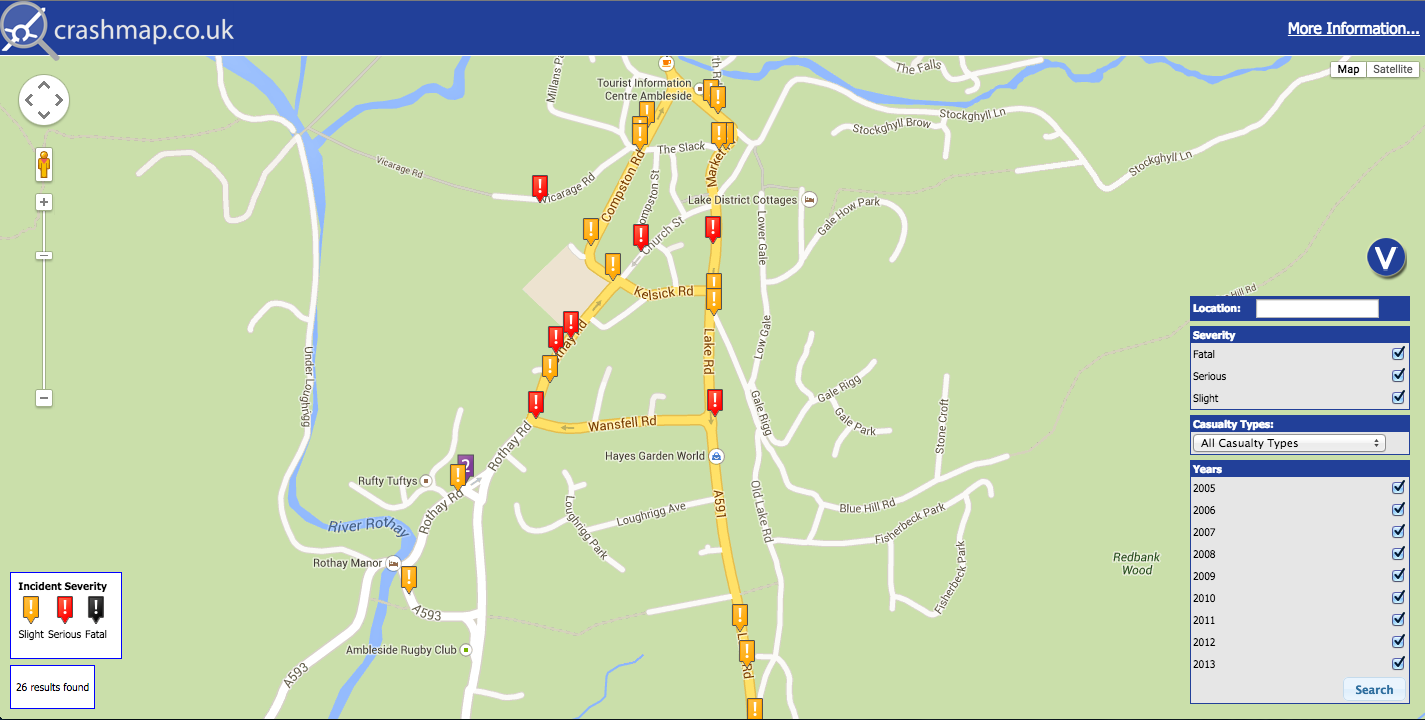
\includegraphics[scale=0.3]{crashmap}
	\caption{Crash Map application}
	\label{fig:crashmap}
\end{figure}

Collision Map \citep{DepartmentforTransport} is similar in purpose to Crash Map. It displays the location of accidents on an interactive map, and also has filters that can be used, including severity, casualty age band and vehicle type (see \autoref{fig:collisionmap}). It differs to Crash Map in that you must select a local highway authority rather than searching for a location or using the map to find it. Clusters of accidents are displayed as one marker on the map, with a number representing how many accidents are in that area. You can reveal the exact location of each accident by zooming in further.

Collision map has several useful features, but has similar limitations to Crash Map. The main advantage of this application is the grouping of accidents to signify hotspots. This makes it very easy to look at an area and see where the most accidents have occurred. A disadvantage in comparison to Crash Map is that you can only use accident data for one year in any search. Like Crash Map, it also lacks the capability of analysing particular routes. This becomes particularly difficult if a route passes through more than one highway authority as you would need to change the search parameters. 

\begin{figure}
	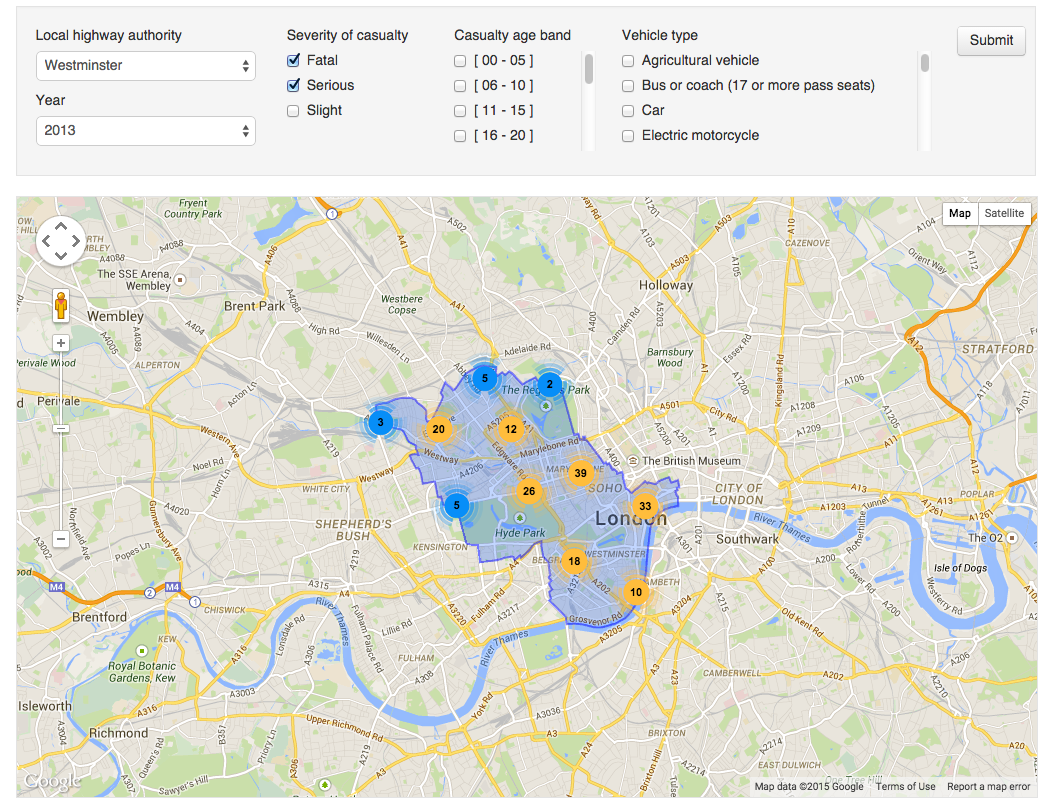
\includegraphics[scale=0.3]{collisionmap}
	\caption{Collision Map application}
	\label{fig:collisionmap}
\end{figure}

Motorcycle Accidents \citep{Mceinsurance} provides an interactive guide to motorcycle accidents in the UK. The aim of this application is to provide motorcyclists with information about where and when it is safest to ride. The application allows you to view statistics about motorcycle accidents on a regional basis (see \autoref{fig:motorcycle}). The application makes use of several fields from the Open Datasets, including road conditions, time of day and severity. For each field, you can view a break down of the data in each region. For example, you can analyse how accidents depend on time of day in London. The application also presents two key facts for each field in order to summarise the data.

The data is presented in a manner that is easy to analyse for any user, and the facts give a concise summary of the findings from the data. This is adequate to serve the application's purpose, but there are limitations that affect the overall usefulness. For example, it is not possible to view specific accident hotspots. The regions cover very large areas, and there is no breakdown of where the accidents occur within these areas.

\begin{figure}
	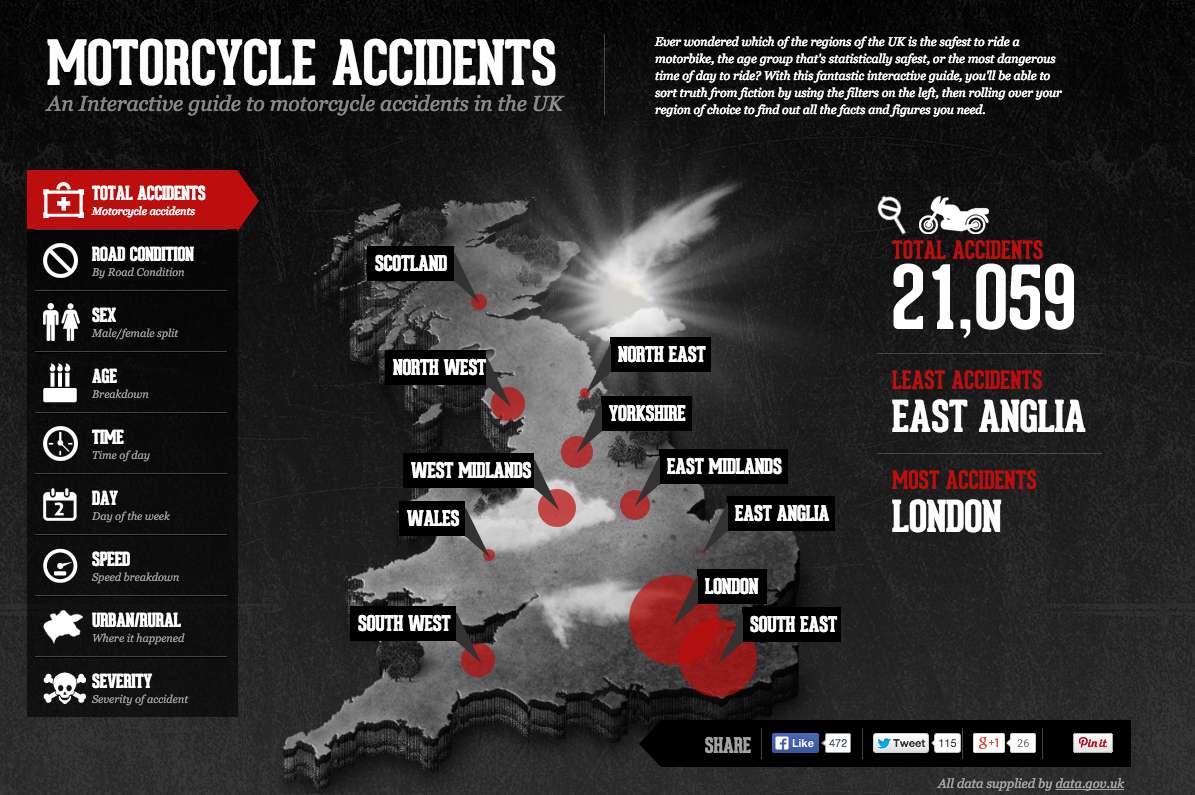
\includegraphics[scale=0.3]{motorcycle}
	\caption{Motorcycle Accidents application}
	\label{fig:motorcycle}
\end{figure}

The final application that I will look at is Walkonomics \citep{Davies}. Walkonomics aims to rate the 'walkability' of streets around the world by combining the views of large groups of people, local communities and Open Data. You can search for a location, and the application will return a list of streets near that location, along with a map displaying markers for each street (see \autoref{fig:walkonomics}). You can then click on a street name in order to find out more information about that street. This page presents a list of reviews for that street, including one from 'Walkobot' which is based on various Open Datasets. Additionally, a user may add a review of their own on this page. 

Walkonomics extends what the other applications have achieved with Open Data. Not only does it use Open Data from different countries, but it also uses different types of data (road safety and crime are mentioned). In addition to this, it combines the use of Open Data with crowdsourcing. Beyond being a web application, Walkonomics is also available to download as an App on both Android and iOS devices.

However, there are some major limitations to this application. For example, when searching for several major cities across the world (including Cardiff, Edinburgh, Paris, Sydney and Los Angeles), no results are found (this behaviour was observed when exploring the application available online on 10/4/2015). It is unclear whether this is a bug or expected behaviour. Additionally, there is no transparency over which Open Datasets are used; it mentions the use of road safety and crime data, but does not specify which countries/states they have obtained this data from. As an application that claims to use data from various different sectors and sources, it should provide a more detailed list of datasets used.

\begin{figure}
	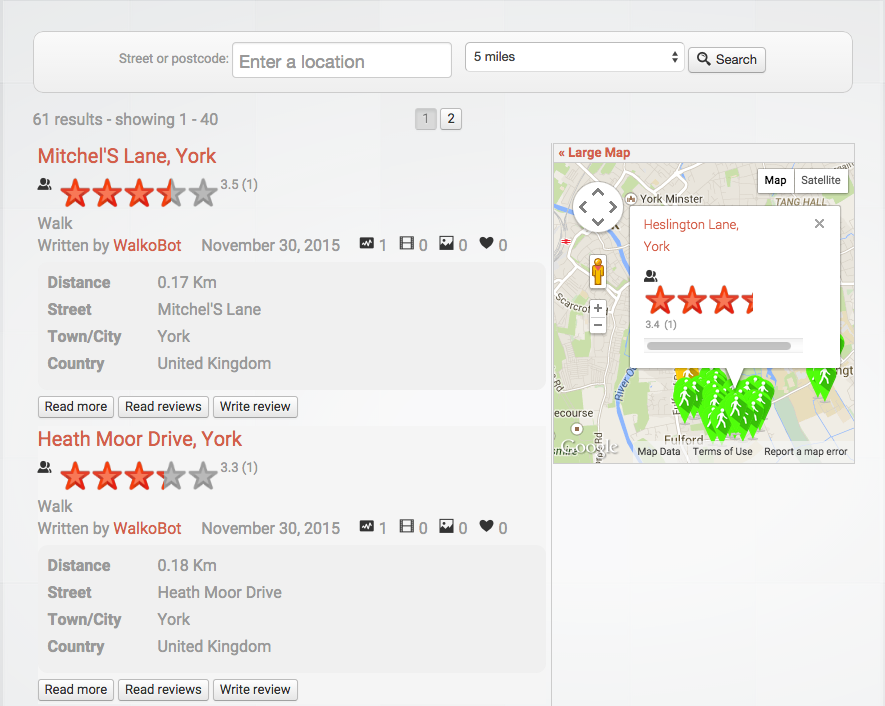
\includegraphics[scale=0.4]{walkonomics}
	\caption{Walkonomics application}
	\label{fig:walkonomics}
\end{figure}

The four applications discussed are compared in \autoref{tab:applications}. The following characteristics were not included in the table as they are common to all four applications:

\begin{enumerate}
  \item The applications are not open source.
  \item The applications are not capable of filtering collisions by route.
\end{enumerate}

As these applications all rely on Open Data, it is disappointing that the developers have not made their code available. The community would benefit greatly from this, as people like myself looking to build new applications would be able to more thoroughly analyse the existing work. By sharing ideas about how to develop such applications, the community can work together to improve them and agree on the best approach.

Another noticeable aspect from this comparison is the similarity between Crash Map and Collision Map. In fact, there are several other applications listed on \textit{data.gov.uk} that are similar to these. This led to the Department for Transport taking Collision Map offline in March 2015, as they felt it offered low value to taxpayers due to the number of alternatives available.  All of these applications operate in the same way; you zoom to an area of the map, and all accidents within that area are displayed. There are no advanced searching facilities available, such as searching for collisions on a particular route only. If you wanted to find such information, you would need to find the route yourself and manually pan the map, counting how many accidents are plotted. Clearly there is room for a new application that provides more advanced features like this.  


\begin{table}[tbp]
   \caption{Comparison of applications that use road safety data}
  \begin{tabular}{ p{2.2cm}  p{3.0cm}  p{2.2cm}  p{2.0cm} p{3.0cm} }
      \textbf{Application} & \textbf{Data} & \textbf{Platform(s)} & \textbf{Mapping API} & \textbf{Data Filters}
    \\Crash Map & UK Road Safety 05-13 & Web & Google Maps & Severity, Casualty Types, Year
	\\Collision Map & UK Road Safety 05-13 & Web & Google Maps & Highway Authority, Year, Severity, Casualty Age, Vehicle Type
	\\Motorcycle Accidents & UK Road Safety 2011 (Motorcycle Only) & Web & N/A & N/A
	\\Walkonomics & Road Safety, Crime & Web, iOS, Android & Google Maps & N/A
  \end{tabular}
  \label{tab:applications}
\end{table}

\section{Web Application Development}

\subsection{Overview}

Jazayeri's study of trends in web application development discusses the area of web application development from a software engineering perspective \citep{Jazayeri2007}. The Web is described as "an attractive playground for software engineers where you can quickly release an application to millions of users and receive instant feedback". It is argued that web applications reach "users that are varied in age, culture, language, education, interest, needs, etc.", and that providing for such varied users poses many interesting challenges. However, whilst all applications may be able to reach such a varied audience, I would argue that most have a specific target audience that the application can be catered to. Hence the challenges of providing for a varied user base is more dependent on the type of application, rather than the platform on which the application is available. 

A major benefit of web applications over desktop applications is the ease in which new versions can be released. In a desktop application, even a small bug fix will require a new version to be installed for all clients. This can lead to numerous issues, as explained by Jazayeri \citep{Jazayeri2007}. In contrast, a web application exists on one server and the browser acts as a universal client. This means that features and bug fixes can be deployed as soon as they are ready, and users will instantly have access to the upgraded application without having to install an update. This leads more kindly to an agile development strategy, as small updates can be released at any time with no impact on users. Desktop applications are more likely to require updates to be grouped together in order to reduce the number of updates that the user must install. However, it is worth noting that some web applications may also require updates to be bundled if they require downtime in order to be applied.  

Web development has been "driven by a move towards open source and standardised components" \citep{Jazayeri2007}. This trend is seen right through web development, from the application itself to the server that it is hosted on. The standard open source server environment used by many is commonly referred to as LAMP. This represents the operating system (Linux), the web server (Apache), the database server (MySQL), and the scripting language (PHP, Perl or Python). The main advantage of a  LAMP environment is that it can be assembled relatively easily and cheaply. PHP, MySQL and Apache are the three most commonly used tools in their respective categories. They have all been developed by programmers within the community who focus on writing features that they want and need \citep{Nixon2009}. As the code is available for all to see and change bugs can be resolved and potential security issues can be prevented before they happen.


\subsection{Programming Languages for Web Application Development}

This section compares and contrasts some of the most popular programming languages used for web applications. The focus is on three of the most popular server-side scripting languages that are used in modern web applications; PHP, Python and Ruby. There is also a discussion of the most popular client-side scripting language, JavaScript.

PHP is a server scripting language designed by Rasmus Lerforf. It is fast, flexible and one of the most popular scripting languages available. According to Netcraft's Web Server Survey of January 2013, PHP was being used by 244M sites at this time \citep{Ide2013}. This equates to 39\% of all sites used in the survey. A large factor behind this popularity is the number of content management systems and ecommerce solutions that are written in PHP; WordPress, Joomla, Drupal, Zencart, osCommerce and Megento account for 32M of these sites. PHP's main advantages include the number of built-in libraries for common web tasks, the ease of learning and use, and its portability \citep{Welling2005}. Its flexible integration with HTML makes client tier integration easy. The main disadvantage of PHP stems from its huge popularity. Because of the huge number of applications authored in PHP, hackers are presented with a "huge and rather attractive attack surface" \citep{Ide2013}. Additionally, due to the open source nature of PHP, it is easier for hackers to find exploits. 

Ruby is a dynamic, imperative object-oriented programming language developed by Yukihiro Matsumoto. Ruby on Rails is a popular framework for web application development based on the model view controller pattern. This framework adds a set of powerful functionalities such as scaffolding, active record, migrations, routing, environments, and many helper functions \citep{Jazayeri2007}. Advantages of Ruby include better security features, pure object-oriented programming, highly readable code and good testing frameworks. Disadvantages include a steep learning curve and a lack of informational resources.

Python was first released in 1991 by Guido van Rossum. In contrast to PHP, it was initially designed as a full-featured general purpose language. It supports multiple programming paradigms, including object-oriented and functional programming. Its design philosophy emphases code readability. Python is quick and easy to learn and it has a large community who provide good support. Disadvantages of Python include its lack of true multiprocessor support and absence of commercial support. 

A comparison of these three languages is presented in \autoref{tab:weblanguages}. The languages have been ranked based on several criterion, with 1 signifying the best rating and 3 the worst. The rankings are based on previous discussion, further research and Klaus Purer's study \citep{Purer2009}. Purer found PHP to be most popular, followed by Python, with Ruby the least popular. GitHut is an online tool that analyses how popular programming languages are on GitHub \citep{Zapponi2014}. It shows that in Q4 of 2014, Python featured in more active repositories than PHP and Ruby. Whilst this suggests that the relative popularity may have changed since Purer's report of 2009, the TIOBE Index for March 2015 still shows PHP above Python \citep{TIOBESoftware2015}. The next comparison is based on the ease with which the language can be learned ('learnability'). These rankings are based on Purer's discussion on readability, and personal opinion from looking at the languages. The rankings for security are based on Purer's conclusion where he found PHP to be slightly behind the others. PHP is mainly criticised for allowing poor programming practices which "result in many security related bugs". All of these languages are open source, which can raise security issues as hackers can use the source code to identify vulnerabilities before attacking sites. 

\begin{table}[tbp]
   \caption{Comparison of PHP, Ruby and Python}
  \begin{tabular}{ p{4.0cm}  p{3.0cm}  p{3.0cm}  p{3.0cm} }
      \textbf{Criterion} & \textbf{PHP} & \textbf{Ruby} & \textbf{Python}
    \\Popularity & 1 & 3 & 2 
    \\Learnability & 2 & 3 & 1
	\\Security & 2 & 1 & 1 
	\\Community & 1 & 2 & 1 
  \end{tabular}
  \label{tab:weblanguages}
\end{table}

The following criteria were not included in the table as the languages were considered to be equal for them:

\begin{enumerate}
  \item Performance.
  \item Database abstraction.
  \item Exception handling.
  \item Available frameworks.
\end{enumerate}

Performance of the languages was compared by Purer, and he considered them too similar to differentiate. He argued that PHP was inferior when it comes to database abstraction and exception handling, as these features hadn't been implemented correctly in some long-living PHP projects. This is an unfair conclusion as PHP does include the features. An unbiased comparison of the three languages should focus purely on the features of the languages, rather than the implementation of the features by some developers. All three languages have highly popular web frameworks with thriving communities. Examples include Laravel for PHP, Rails for Ruby and Django for Python.

Client-side JavaScript combines "the scripting ability of a JavaScript interpreter with the Document Object Model (DOM) defined by a web browser" \citep{Flanagan2006a}.This means that it can add behaviour to otherwise static web content. This technology is the core of web development techniques such as Dynamic HTML and architectures such as Ajax (Asynchronous JavaScript and XML). JavaScript helps reduce server usage, as functions that were typically performed on the server can be done on the client (e.g. form validation) \citep{Jazayeri2007}. Browsers are able to provide more responsive operations to the user by pushing some of the client-server communication to the background while the application is still interactive. This can be achieved using Ajax to introduce an intermediary 'engine' between the user and the server \citep{Garrett2005}. Every user action that would normally generate a HTTP request takes the form of a JavaScript call to the Ajax engine instead. If the engine needs something from the server to respond (e.g. retrieving new data), the engine makes those requests to the server asynchronously without interrupting the user's interaction with the application. 


\subsection{Model-View-Controller}

A large number of contemporary web frameworks make use of the Model-View-Controller (MVC) design pattern. The Model is the application object, the View is its screen representation, and the Controller defines the way the user interface reacts to user input \citep{Gamma1995}. The MVC pattern had been popular in software engineering for many years before it was realised that it could be applied just as well to web applications \citep{Jazayeri2007}.  The main problem with using the MVC design pattern when developing web applications is that the application must be partitioned between the client and the server \citep{Leff2001}.

Morales-Chapar et al. provide an interesting discussion on the different implementations of MVC in web applications \citep{Morales-Chaparro2007}. This paper focuses on "large-scale web applications which are data dynamic and typically written in two programming languages", much like my application will be. A case study is used to compare the advantages and disadvantages of server-side MVC with two mixed client-side and server-side MVCs. 

Server-side MVC is derived from desktop MVC, in that all components are usually programmed in the same language and the server runs all computations and operations. It is pointed out by Morales-Chaper et al. that this approach is useful when "applications capabilities requirements are poor at client side (e.g. mobile browsers without JavaScript functionality) or when application necessity is only to display information with low levels of user interaction". It is worth consideration that this paper was published in 2007, and since this time mobile devices and browsers have advanced significantly, so the first advantage given is of little relevance now. The disadvantages of this approach include the incapability of updating part of a view, increased bandwidth usage and the higher server usage due to the server validating forms, amongst other things.  

The first mixed client-side and server-side MVC discussed by Morales-Chapar et al. was designed with a focus on resolving the previously raised issues. This MVC design involves dividing the Controller and View between the server and client, whilst leaving the model at server-side. In this system, some processing is now done on the client-side; for example, form validation using JavaScript. They raise the issue of different browsers and operating systems causing issues when accessing UI elements. Whilst the situation has improved since 2007, there still exists the issue of browsers not implementing exactly the same standard specifications. This approach still has the disadvantage of not being able to retrieve data asynchronously without refreshing the page. Without a model on the client-side, there are limitations on providing high interaction levels and data manipulation becomes more difficult. In comparison with the pure server-side approach, there is an increase in computation time and complexity due to the logic now present on client-side. 

The second mixed client-side and server-side MVC discussed by Morales-Chapar et al. is similar to the previous design, but with part of the model on client-side. This design addresses the issue of not being able to retrieve data asynchronously without refreshing the page, by allowing for the use of Ajax. Limitations of this design include slower computation for tasks requiring access to the server, difficulty of designing a client-side model that is compatible with all browsers, and increased overhead on communications among MVC design elements. 


\section{Software Development Methodologies}

This section features a discussion of some popular software engineering methodologies that were considered for this project. The discussion focuses on those that are most beneficial to a project like this one, i.e. a web application developed by one person in a limited time frame. 

Pfleeger and Atlee define software engineering as "an approach that combines computer science (which is made up of theories and computer functions) and the customer (who provides the problem to be solved) to develop a set of tools and techniques to solve problems" \citep{Pfleeger}. Software engineering methodologies can be defined as a group of methodologies used in the development of applications. Methodologies give details of "what should be done in each phase of the software development process" \citep{Mnkandla2009}. They do not necessarily give details of how things should be done, allowing for some tuning by those using them. 

Agile software development is a conceptual framework for undertaking software engineering projects \citep{ITKnowledgePortal}. Agile methods generally try to minimise risk by developing software in iterations, which typically last one to four weeks. Each iteration of the project is like its own project, featuring its own planning, requirement analysis, design, coding, testing and documentation phases. At the end of each iteration, a new working version of the application should be available. The team is then able to re-evaluate the project priorities ahead of the next iteration. Agile methods emphasise working software as a primary measure of progress.

Scrum is a software-management process for iterative-incremental software development projects. Scrum relies on self-organisation, with the team deciding what to do while management removes roadblocks \citep{Faridani2011}. Scrum is focused on frequent intermediate delivers with working functionality. Alongside this, there are frequent risk and mitigation plans produced by the development team. There are daily 'scrums', where the development team meet up to explain progress, describe upcoming work and raise obstacles. 

Extreme Programming is an iterative and incremental development methodology. Key practices of Extreme Programming include: making a rough plan quickly and refining it as thing become clearer, test driven development, re-factoring code, continuous integration of code, and an on-site customer to clarify requirements and make crucial business decisions \citep{Faridani2011}. 

It is clear that the methodologies described are designed for team projects, rather than an individual project like this one. However, there are useful concepts that can be taken from each of them and applied to this project. It will be advantageous to split development work into iterations. This will encourage the delivery of a new, functional version of the application at regular intervals. This approach is particularly beneficial if there are issues to developing a complex piece of functionality in a later iteration, as there will still be a functional version of the application from the previous iteration. 


\section{Design of Interactive Applications}

A key aspect of designing a successful web application involves focusing on user interaction. User-centred is a process in which the needs, wants, and limitations of end users of a product are given extensive attention at each stage of the design process. In this section, I will discuss some design principles that will help me to develop a user-friendly application. 

Rogers et al. state that interaction design is about "developing interactive products that are easy, effective and pleasurable to use from the users' perspective" \citep{Rogers2011}. They define the process of interaction design as 4 basic activities: establishing requirements, designing alternatives, prototyping and evaluating. These activities are intended to inform one another and to be repeated. The repetition is necessary as, for example, you may find that new requirements are needed following feedback in the evaluation phase. Cooper et al. explain the concept of goal-directed design as designing and constructing products in such a way that the people who use them achieve their goals \citep{Cooper2007}. The users should be "satisfied, effective, and happy". The goal-directed design process is divided into six phases: research, modelling, requirements definition, framework definition, refinement and support. 

Some key design principles from these books are presented in \autoref{tab:designprinciples}.

\begin{table}[tbp]
   \caption{Interactive Design Principles}
  \begin{tabular}{ p{2.0cm}  p{9.0cm}  p{3.0cm}   }
      \textbf{Design Principle} & \textbf{Description} & \textbf{Source(s)} 
    \\Usability Goals & There are six goals: effectiveness, efficiency, safety, utility, learnability and memorability. Typically assessed using questions. Developers can ask these questions during design process to be alerted early on about any design problems that they have not considered. It is possible to establish quantifiable criteria for some usability goals. For example; time to complete a task (efficiency) and time to learn a task (learnability).  &  Interaction Design: Beyond Human Computer Interaction \citep{Rogers2011}.
     \\User experience goals & Cover a range of emotions and felt experiences, both desirable and undesirable. Concerned with how users experience an interactive product from their perspective, rather than assessing how useful a system is from its own perspective. Assessed using questions.  &  Interaction Design: Beyond Human Computer Interaction \citep{Rogers2011}.
       \\Personas & Descriptive models of users created based on research. Cooper et al. state that personas "provide us with a precise way of thinking and communicating about how users behave, how they think, what they wish to accomplish, and why". They are not real people, but based on the behaviours and motivations of real people. Personas are depicted as specific individuals, but they also represent a class or type of user of a specific interactive product.  &  About Face 3 : The Essentials of Interaction Design \citep{Cooper2007}.
       \\Scenarios & A means of imagining ideal user interaction. Persona-based scenarios are "concise narrative descriptions of one or more personas using a product to achieve specific goals". This lets a designer work with a story describing an ideal experience from the persona's perspective, with a focus on how they think and behave. These scenarios help drive requirement definition.  &  About Face 3 : The Essentials of Interaction Design \citep{Cooper2007}.
       \\Requirement Definition & Requirements specify "what information and capabilities our personas require to accomplish their goals". The requirement definition process consists of five steps: creating problem and vision statements, brainstorming, identifying persona expectations, constructing context scenarios and identifying requirements. &  About Face 3 : The Essentials of Interaction Design \citep{Cooper2007}.
  \end{tabular}
  \label{tab:designprinciples}
\end{table}

The concepts discussed thus far will help to design a system that offers the functionality required by users. Another important aspect of designing interactive applications involves creating a user interface that that is satisfying to use. To help with this, there are some common design conventions applied to most web applications that can be followed. Lynch and Horton discuss some of these conventions in 'Web Style Guide' \citep{Lynch2009}. The first of these conventions is 'restraint and simplicity'. This involves focusing on critical functions of an application and avoiding all "nice-to-have and easy-to-add features". The critical features should be addressed with a design that is uncluttered by unnecessary elements. Another key convention involves guiding interaction by making the design self-explanatory. A good design should guide users through the functional elements of a page. Instructions, labels, prompts and design patterns can be used to explain what is expected and how the page works. Feedback is crucial to a well designed application. For example, if an error has occurred, it is important to alert the user with a clear error message explaining why an error has occurred and how the user can resolve it. 

\section{Mapping APIs}

A fundamental objective of this project involves using an interactive map to analyse collision hotspots. This will require the use of a mapping API. It is important that the API used is capable of finding a route, analysing whether a collision is on the route, and visualising collision density. This section features an analysis of some of the most popular JavaScript mapping APIs that are available; Google Maps, Bing Maps and OpenLayers.  

Google introduced the first mapping API in 2005. The Google Maps API \citep{Google} enables the overlaying of data on top of tiled map layers from Google Maps. It brings the look and feel of Google Maps, that many internet users are already familiar with, to third-party applications. The API can be used by most websites free of charge, but charges will incur if the site consistently generates high traffic (25,000 map loads per day for 90 consecutive days). Google provide a number of services and libraries that can be used by developers looking for advanced functionality. Services include directions, geocoding and street view. There is a geometry library that provides "utility functions for the computation of geometric data on the surface of the Earth" (e.g. you can determine whether a given point is near a line). The visualisation library includes 'heat map layer' functionality for visualising data intensity at geographical points.

Microsoft's Bing Maps API \citep{Microsoft} is similar in scope to Google's API. Bing Maps also offers a free usage tier, with a limit of 125,000 cumulative billable transactions within any 12-month period. It was released five years after the Google Maps API and is still behind in terms of functionality offered, hence its lower popularity. There is a considerable amount of documentation available online, but it isn't structured or presented as well as Google's, making it far more frustrating to use. The core API doesn't have advanced geometry and visualisation libraries like Google Maps API. However, it is possible to import third party modules that offer some of this functionality (such as heat maps). 

OpenLayers \citep{OpenLayers} is an open source mapping API that was initially released in 2006. It is very flexible and powerful but also complex and large. It has an extensive collection of documentation and samples, some of which can be difficult for beginners to grasp. It has a large developer community behind it who have provided plenty of tips and example uses. OpenLayers does not have its own directions service, making route calculation a difficult task. OpenLayers is far more complex than the alternatives and more suitable for GIS experts. A lot of the extra functionality that it offers is not required for this project.

From this analysis, it is clear that Google Maps offers the most benefits to a project like this. It was created first, and has consistently grown to keep ahead of the competition. Detailed documentation is available online, and there is a large community of developers who are willing to provide support. The heat map functionality will be useful for visualising the density of collisions, thus highlighting collision hotspots. It is also notable that three of the existing applications analysed use the Google Maps API; demonstrating its popularity in the field.

\chapter{Problem Analysis}

\section{Introduction}

This chapter will analyse the problem presented by the project, with a focus on using the goal-directed design process \citep{Cooper2007}. Firstly, personas will be created to represent potential users of the application. Scenarios describing how these personas would ideally interact with the application in order to achieve their goals will then be written. Finally, the functional and non-functional requirements of the application will be defined, using the scenarios and findings of the literature review as motivation. 

\section{Personas} 

Unfortunately there was not enough time to perform the necessary fieldwork in order to make 'rigorous' personas. Therefore, 'provisional' personas were created based on available data and best guesses about behaviours, motivations and goals. It is stated by Cooper et al. that the use of these provisional personas has proven more successful than not using user models at all \citep{Cooper2007}. 

Cooper et al. warn of some potential issues to avoid when creating provisional personas. It is important to avoid focusing on the wrong design target. Even if you are focusing on the correct target, you must be careful to ensure that key behaviours that could differentiate the product are not missed. It is important to focus on behaviours and motivations rather than demographics.

Two personas have been created and are presented in \autoref{fig:personaA} and \autoref{fig:personaB}. Aspects of Persona A were based on information provided by West Sussex Council about the process used to improve road safety\citep{WestSussexCountyCouncil}.

\begin{figure}
	\begin{framed}
 		Linda is a member of the transport department in West Sussex County Council. Linda has good IT skills after taking several training courses and she is familiar with road safety data. One of the main objectives in her job is to improve road safety in the county. Due to the limited resources of the council, route improvements must be prioritised by Linda. In order to do this, she uses the council's 'accident location map' to find the number of casualties per kilometre on a route. This is a slow and tedious task, as she must manually pan the map to find each accident on the route before clicking on each one to find the details. Linda finds this process frustrating and boring, so often assigns the task to a junior member of staff. She believes that resources could be better spent on other tasks if there was an application that automated the process.
  	\end{framed}
  \caption{Persona A: Linda}
  \label{fig:personaA}
\end{figure}

\begin{figure}
	\begin{framed}
 		John is the owner of a company that delivers food products from manufacturers to supermarkets. John joined the company after graduating from his law and finance degree 12 years ago, before eventually inheriting it from this late father. John considers himself a 'tech enthusiast' and is always looking to innovate how the company do day-to-day tasks. He has recently become interested in Open Data, and how he can use it to benefit his business. He is curious about using road safety data to find out about accident hotspots, so that his drivers can avoid them. He hopes that this will reduce the risk of late deliveries due to traffic delays, whilst also reducing the risk of one of his drivers being involved in a collision. 	\end{framed}
  \caption{Persona B: John}
  \label{fig:personaB}
\end{figure}


\section{Scenarios}

Context scenarios are used to "explore, at a high-level, how the product can best serve the needs of the personas" \citep{Cooper2007}. These scenarios are used to imagine an ideal user experience whilst intentionally being broad and relatively shallow in scope.

The context scenario presented in \autoref{fig:scenarioA} describes how Linda would use the application. Scenario B (see \autoref{fig:scenarioB}) describes an ideal user experience for John.

\begin{figure}
	\begin{framed}
		The new financial year has recently began, and the West Sussex County Council have a new budget to allocate to road safety improvements. The council needs to prioritise the most dangerous routes in the county by using STATS19 data to see where the most casualties have occurred. Linda did this analysis last year, but the council wants new analysis to be done, making use of the latest data released by the Department for Transport.
		
		Linda accesses an online application for analysing road safety on her work computer. She enters the first route's start location and destination, and chooses to search all collision data for the last 3 years. The application returns the weighted casualties per kilometre for the route. Linda makes a note of this number, and then repeats the process for all routes. She is now able to suggest which routes need safety improvements based on these figures.
  	\end{framed}
  \caption{Scenario A: Linda using the application}
  \label{fig:scenarioA}
\end{figure}

\begin{figure}
	\begin{framed}
 		John's company have recently acquired a lucrative contract to deliver fresh goods to a large supermarket chain. There is a strict deadline for when the food must be delivered each day, with little allowance for delays. In order to minimise risk, John wants his drivers to avoid roads with accident hotspots.
 		
 		John logs in to his laptop and accesses an online application for analysing road safety. He begins by inputting the postcodes for the manufacturer and the supermarket. He then decides to only include collisions from the last two years as he believes older data will be less relevant due to road changes. He decides to include serious and fatal collisions only, as these are likely to cause lengthy delays. After John submits his search, the application displays a map with a visual representation of where collisions have occurred on the route. John notices an accident hotspot on the route, and instructs his drivers to take a minor diversion in order to avoid it.
  	\end{framed}
  \caption{Scenario B: John using the application}
  \label{fig:scenarioB}
\end{figure}


\section{Requirement Definition}

Requirements can now be derived based on project objectives, findings of the literature review, personas and scenarios, software engineering best practices and software quality standards. The requirements will specify \textit{what} the application should do, and the design chapter will focus on \textit{how} this can be achieved.

\subsection{Functional Requirements}

The functional requirements of the system are presented in \autoref{tab:FunctionalReqs}. The requirements have been ranked by importance to help prioritise them during the development phase. A brief justification of each requirement will now follow. 

The project objectives make FR1 an absolute necessity, as using this data is fundamental to the project. The analysis of existing applications in the literature review led to the formation of FR2. This addresses the project objective of developing a unique piece of functionality that makes the application stand out. Additionally, both scenarios have demonstrated the need for this functionality. Scenario A raises the need for consecutive searches (FR6) and collision statistics as mentioned in FR4 and FR5. The need for additional data filters, as described in FR3 and FR7, is justified by each of the scenarios. It is also notable that two of the existing applications analysed included these filters. FR8 addresses the project objective of highlighting accident hotspots, and also satisfies the user goal described in Scenario B. FR9 can be inferred from Scenario B, as this functionality would help John in planning the diverted route. The implementation of FR10 would help satisfy the project objective of establishing a framework for web applications interacting with Open Data.

\begin{table}[tbp]
\caption{Functional Requirements}
\begin{tabular}{| p{1.5cm} | p{7.5cm} | p{2cm} |}
	\hline
	\textbf{ID} & \textbf{Description} & \textbf{Importance} \\ \hline
	FR1 & The application should use road safety data published by the UK Department for Transport. & High \\ \hline
	FR2 & The application should find a route between two user-entered locations and find collisions on this route. & High \\ \hline
	FR3 & Users should be able to filter collisions included in results by year. & Medium \\ \hline
	FR4 & The application should calculate and present some statistics using the 'accidents' dataset, such as number of collisions. & High \\ \hline
	FR5 & The application should calculate and present some statistics using the 'casualties' dataset, such as 'weighted casualties per kilometre'. & Medium \\ \hline
	FR6 & The user should be able to immediately submit a new search after a previous search has finished. & High \\ \hline
	FR7 & Users should be able to filter collisions included in results by severity. & Medium \\ \hline
	FR8 & Collision density should be represented visually on an interactive map in order to highlight hotspots. & High \\ \hline
	FR9 & The application should suggest lower risk routes for the specified journey. & Low \\ \hline
	FR10 & The datasets used should be automatically updated when new datasets are released. & Low \\ \hline
\end{tabular}
\label{tab:FunctionalReqs}
\end{table}

\subsection{Non-functional Requirements}

The non-functional requirements of the system are presented in \autoref{tab:NonFunctionalReqs}. These requirements have also been ranked by importance. A brief justification of each requirement will now follow. 

Most of these requirements were inspired by software quality standards \citep{ISO9126}. NFR3, NFR4 and NFR6 all address the usability standard. NFR5 focuses on efficiency. In reality, most searches should take under 5 seconds, but if a user searches for all collisions on a very long route, there will be thousands of results to analyse. NFR7 addresses the maintainability standard. Finally, NFR1 is inspired by the portability standard.

\begin{table}[tbp]
\caption{Non-functional Requirements}
\begin{tabular}{| p{1.5cm} | p{7.5cm} | p{2cm} |}
	\hline
	\textbf{ID} & \textbf{Description} & \textbf{Importance} \\ \hline
	NFR1 & The application should be compatible with the latest (desktop) versions of Google Chrome, Mozilla Firefox and Internet Explorer. & High \\ \hline
	NFR2 & The application should be open source. All code should be available on GitHub. & High \\ \hline
	NFR3 & Users should be able to understand how to use the application without external assistance. & High \\ \hline
	NFR4 & Results of data analysis must be presented in a user-friendly manner. & High \\ \hline
	NFR5 & The time taken to perform data analysis should never exceed 30 seconds. & Medium \\ \hline
	NFR6 & The system's progress should be displayed whilst data analysis is being performed. & High \\ \hline
	NFR7 & Data model should allow new datasets to be added to the application in the future. & Medium \\ \hline
\end{tabular}
\label{tab:NonFunctionalReqs}
\end{table}


\chapter{Design}

\section{System Architecture}

\subsection{LAMP}

\subsection{UML Diagram}

\section{Development Process}

\section{Technology Overview}

\subsection{PHP}

\subsection{MySQL}

\subsection{Google Maps API}

\subsection{Version Control System}

\section{Interface Design}

\subsection{Wireframes}

\section{Summary}

\chapter{Implementation and Testing}

\section{Components}

\section{Techniques}

\section{Testing}

\section{Summary}

\chapter{Evaluation}

\section{Discussion}

\section{Usability}

\section{Maintainability}

\section{Limitations}

\chapter{Conclusions}

\section{Lessons Learnt}

\section{Future Work}


\bibliography{library}


\end{document}
